\begin{frame}
  \frametitle{Markov chain Monte Carlo}
  Markov chain Monte Carlo methods allow sampling from a
  probability distribution whose form is not explicitly known.
  \vspace{3em}

  These methods work by constructing a Markov chain whose stationary
  distribution is equal to the probability distribution.
\end{frame}

\begin{frame}
  \frametitle{Metropolis-Hastings Algorithm}
  \begin{center}
    Metropolis-Hastings draws samples from any probability distribution $p(x)$, as long as a
    function $f(x) \propto p(x)$ is known.
    \vspace{3em}

    This is very useful in Bayesian inference for non-conjugate posteriors
    in multi-dimensional vector spaces.
    \[p(x|h) \propto p(h|x) p(x)\]
  \end{center}
\end{frame}

\begin{frame}
  \frametitle{Overview of Metropolis-Hastings}
  \begin{columns}
    \begin{column}{0.4\textwidth}
      \begin{itemize}
      \item We move from $x_t$ to a new state $x'$ based on the value of
        $\frac{f(x')}{f(x_t)} = \frac{p(x')}{p(x_t)}$
      \item This mimics shape of $p(x)$ by spending more time in the regions where $f(x)$ is larger.
      \end{itemize}
    \end{column}
    \begin{column}{0.6\textwidth}
      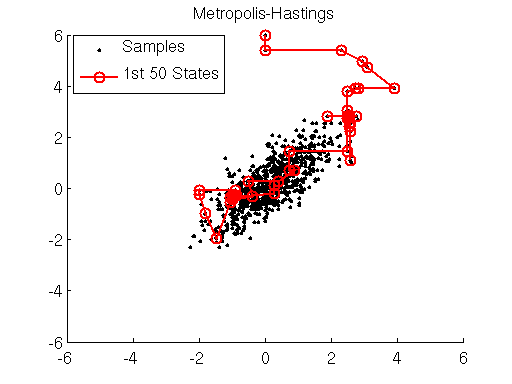
\includegraphics[width=3in]{img/metropolis-hastings}
    \end{column}
  \end{columns}
\end{frame}

\begin{frame}
  \frametitle{Transition to new state}
  \begin{enumerate}
    \item Choose a potential new state $x'$ around $x_t$ based on the proposal
      distribution (often a Gaussian)
    \item Define $a = \frac{f(x')}{f(x_t)} = \frac{p(x')}{p(x_t)}$
    \item If $a \geq 1$, $x_{t+1} = x'$. Otherwise, 
      \[x_{t+1} = 
      \begin{cases}
        x', & \text{with probability } a \\
        x_t, & \text{with probability } 1 - a
      \end{cases}\]
  \end{enumerate}
\end{frame}

\begin{frame}
  \frametitle{Proposal Distribution}
  \begin{itemize}
  \item The proposal distribution is used to choose $x'$ from $x_t$.
  \item The distribution must be symmetric about $x_t$ -- typically a
    Gaussian distribution centered about $x_t$ is chosen.
  \item The variance of the distribution crucial in determining whether
    Metropolis-Hastings will return a representative sample.
  \end{itemize}
\end{frame}

\begin{frame}
  \frametitle{Issues to note with Metropolis-Hastings}
  \begin{itemize}
    \item A burn-in is required to avoid bias based on the initial state $x_0$.
      Often the burn-in will need to be over $1000$ samples.
    \item To minimize auto-correlation between samples, take only every $n^{\text{th}}$
      sample from the samples remaining after burn-in.
  \end{itemize}
\end{frame}